% THIS IS SIGPROC-SP.TEX - VERSION 3.1
% WORKS WITH V3.2SP OF ACM_PROC_ARTICLE-SP.CLS
% APRIL 2009
%
% It is an example file showing how to use the 'acm_proc_article-sp.cls' V3.2SP
% LaTeX2e document class file for Conference Proceedings submissions.
% ----------------------------------------------------------------------------------------------------------------
% This .tex file (and associated .cls V3.2SP) *DOES NOT* produce:
%       1) The Permission Statement
%       2) The Conference (location) Info information
%       3) The Copyright Line with ACM data
%       4) Page numbering
% ---------------------------------------------------------------------------------------------------------------
% It is an example which *does* use the .bib file (from which the .bbl file
% is produced).
% REMEMBER HOWEVER: After having produced the .bbl file,
% and prior to final submission,
% you need to 'insert'  your .bbl file into your source .tex file so as to provide
% ONE 'self-contained' source file.
%
% Questions regarding SIGS should be sent to
% Adrienne Griscti ---> griscti@acm.org
%
% Questions/suggestions regarding the guidelines, .tex and .cls files, etc. to
% Gerald Murray ---> murray@hq.acm.org
%
% For tracking purposes - this is V3.1SP - APRIL 2009

\documentclass{acm_proc_article-sp}
\usepackage[ruled,vlined]{algorithm2e}
\begin{document}

\title{Search for Maximal Unique Matches in Multi-core architectures}

\numberofauthors{4} %  in this sample file, there are a *total*
% of EIGHT authors. SIX appear on the 'first-page' (for formatting
% reasons) and the remaining two appear in the \additionalauthors section.
%
\author{
\alignauthor Julio C\'esar Garc\'ia Vizca\'ino\\
       \affaddr{Computer Architecture and Operating System}\\
       \affaddr{Campus UAB, Edifici Q, 08193}\\
       \affaddr{Bellaterra (Barcelona), Spain.}\\
       \email{juliocesar.garcia@caos.uab.es}
\alignauthor Juan Carlos Moure\\
       \affaddr{Computer Architecture and Operating System}\\
       \affaddr{Campus UAB, Edifici Q, 08193}\\
       \affaddr{Bellaterra (Barcelona), Spain.}\\
       \email{juancarlos.moure@uab.es}
\alignauthor Antonio Espinosa\\
       \affaddr{Computer Architecture and Operating System}\\
       \affaddr{Campus UAB, Edifici Q, 08193}\\
       \affaddr{Bellaterra (Barcelona), Spain.}\\
       \email{antonio.espinosa@caos.uab.es}
\and  % use '\and' if you need 'another row' of author names
\alignauthor Porfidio Hern\'andez\\
       \affaddr{Computer Architecture and Operating System}\\
       \affaddr{Campus UAB, Edifici Q, 08193}\\
       \affaddr{Bellaterra (Barcelona), Spain.}\\
       \email{porfidio.hernandez@uab.es}
}
\date{30 July 1999}
% Just remember to make sure that the TOTAL number of authors
% is the number that will appear on the first page PLUS the
% number that will appear in the \additionalauthors section.

\maketitle
\begin{abstract}
  Maximal Unique Matches are common substrings that match a reference and a query genome. They are exact, unique and maximal. The search of MUMs in large genomes is a heavy and repetitive task, so there is a fair chance of parallelize and execute this search in multi-core architectures. This research resembles an approach to find MUMs in genomic sequences and comparing the search in two data structures within multi-core architectures. The reference genome is indexed by using a suffix tree or enhanced suffix array in main memory and then parallelized algorithm finds the MUMs of query genome which is readed by several threads in chunks of fixed size. This approach is based on MUMmer, a genome alignment tool, which is able to find Maximal Unique Matches (MUMs). 
\end{abstract}

% A category with the (minimum) three required fields
\category{H.4}{Information Systems Applications}{Miscellaneous}
%A category including the fourth, optional field follows...
\category{D.2.8}{Software Engineering}{Metrics}[complexity measures, performance measures]

\terms{Theory}

\keywords{Indexed Search, Bioinformatics, Maximal Unique Match, Multi-core architectures, Parallelization}

\section{Introduction} 
Modern sequencing and computational technologies and advances in bioinformatics has made whole genome sequencing possible. One resulting challenge is the fast alignment of whole genomes. Dynamic programming is too slow for aligning two large genomes. 

One very successful approach to perform whole genome alignment is based on identifying ``maximal unique matches'', which is based on the assumption that one expects to substrings occurring in two similar genomes.
Maximal unique matches (MUMs) are almost surely part of a good alignment of the two sequences and so the whole genome alignment problem can be reduced to aligning the sequence in the gaps between the MUMs.

\newdef{definition}{Definition}
\begin{definition}
Assume we are given two sequences R,Q $\in \Sigma^*$, and a number L > 0. The maximal unique matches problem (MUM-problem) is to find all sequences u $\in \Sigma^*$ with: $|u|\geq L$, u occurs exactly once in R and once in Q, and for any character a $\in \Sigma^*$ neither ua nor au occurs both in R and Q.
\end{definition}

The problem of searching maximal unique matches for a minimum length between a reference string and a query string has been
identified in several applications, one of them is MUMmer \cite{Delcher2003}. MUMmer's algorithm can perform searches of maximal unique matches (MUMs), although
with a high use of main memory to store the reference string and a null use of multi-core architectures.

\section{Related work}
Search of Maximal Unique Matches to do Whole Genome Alignment was proposed in \cite{Delcher1999}. There have been some previous work in the parallelization of search of matches in genomic data, like \cite{OguzhanKulekci2011,Mongelli,Kouzinopoulos2005}, however these works are focused in fixed patterns and read alignment. On the other hand, there have been achievements in parallelization of Whole genome alignment like \cite{Meng2005}. The parallelization of searching MUMs with a full-text index data structure is a research field not covered very deep, there is only one approach in \cite{Encarnac2011} but without access to source code to check their implementation and it is more focused with GPU and CPU hybrid architectures and suffix array. There are other implementations to search Maximal exact matches with threads in \cite{Vyverman2013,OguzhanKulekci2011,Khan2009,OhlebuschGK10}

\section{Preliminaries}
Let's assume the reference string $R[0,\ldots, n − 1]$ of size n over an alphabet $\Sigma={ \$, A, C, G, T}$ which has a sentinel character $R[n − 1] = \$$ that occurs nowhere else in the string and is lexicographically less than all the characters that occur in the alphabet. The suffixes of the reference string are zero indexed by their position in the original string by a full-text index data structure like a suffix tree or a suffix array. 

\begin{definition}
A suffix tree, $ST$, for an n-character string $R$ is a rooted directed tree with exactly $n$ leaves numbered 0 to n. Each internal node, other than the root, has at least two children and each edge is labeled with a nonempty substring of $R$. No two edges out of a node can have edge-labels beginning with the same character. For any leaf $i$, the concatenation of the edge-labels on the path from the root to leaf $i$ exactly spells out the suffix of $R$ that starts at position $i$. That is, it spells out $R[i\ldots n]$. \cite{Gusfield1997}.
\end{definition}
\begin{definition}
Given an n-character string $R$, a suffix array, $SA$, for $R$ is an array of the integers in the range 0 to $n$, specifying the lexicographic order of the $n$ suffixes of string $R$. \cite{Gusfield1997}.
\end{definition}
A search for a MUM between a Reference, $R$ of length $n$, and Query, $Q$ of length $m$, genome can be done in a suffix tree in $O(n+m)$ time and in a suffix array in $O(n\log m)$ time. However is possible to improve the search for MUMs algorithm in a suffix array by using: an inverse suffix array, a LCP-table and a child table. These improvements give a $O(m)$ time \cite{Abouelhoda2004} to search for MUMs in a suffix array.
\begin{definition}
An inverse suffix array, $ISA$, is a table of size $n+1$ such that $ISA[SA[q]]=q$ for any $0\geq q\geq n$. \cite{Abouelhoda2004}.
\end{definition}
\begin{definition}
A LCP-table, $LCP$, is an array of integers from 0 to n. Where $LCP[0]=0$ and $LCP[i]$ is the length of the longest common prefix of $SA[i-i]$ and $SA[i]$ for $1\geq i \geq n$. \cite{Abouelhoda2004}.
\end{definition}
\begin{definition}
A child table, CHILD, is a table of size $n+1$ indexed from 0 to n and each entry contains three values: up, down, and nextlIndex. These values are defined as follows: 

CHILD[i].up = $min\{q\in [0\ldots i-1]|LCP[q]>LCP[i]\;and\;\\
\forall k\in[q+i\ldots i-1]:LCP[k]\geq LCP[q]\}$,

CHILD[i].down = $max\{q\in[i+1\ldots n]|LCP[q]>LCP[i]\\
and\;\forall k\in[i+1\ldots q-1]:LCP[k]\geq LCP[q]\}$,

CHILD[i].nextlIndex = $min\{q\in[i+1\ldots n]|LCP[q]=LCP[i]\\
and\;\forall k\in[i+1\ldots q-1]:LCP[k]>LCP[i]\}$.
\end{definition}
To simulate a traversal of a suffix tree on an enhanced suffix array we require the child table. In order to perform the traversal we get an interval $l-$interval $[i..j]$ and a character $a\in \Sigma$ as input and returns the child interval $[l..r]$ of $[i..j]$ whose suffixes have the character $a$ at position $l$. Note that all the suffixes in $[l..r]$ share the same $l-$character prefix because $[l..r]$ is a subinterval of $[i..j]$. This process is performed in $O(|\Sigma|)$ time.

Once we have defined the resources used to index a Reference genome, we need to answer the question: Where are the MUMs of $R$ and $Q$ of some minimum length $L$? We show the algorithms used to answer this question using a Suffix Tree and a Enhanced Suffix Array.

\linesnumbered
\begin{algorithm}
  \dontprintsemicolon
  \SetKwInOut{Input}{input}
  \SetKwInOut{Output}{output}
  \SetKwData{R}{R}
  \SetKwData{Q}{Q}
  \SetKwData{Len}{L}
  \SetKwData{Length}{length}
  \SetKwData{Leaf}{leaf}
  \SetKwData{MUMs}{MUMs}
  \SetKwFunction{TraverseSuffixTree}{TraverseSuffixTree}
  \SetKwFunction{isLeafNode}{isLeafNode}
  \SetKwFunction{saveMUMcand}{saveMUMcand}
  \SetKwFunction{cleanMUMcand}{cleanMUMcand}
  \Input{\R, \Q, \Len}
  \Output{List of \MUMs of \Length$\geq$ \Len, with start position in \R and \Q and \Length}
  \Begin{
  Build suffix tree for $R$ genome\;
  \ForEach{position $i\in Q$}{
  \Length$\leftarrow$ \TraverseSuffixTree{Q[i]}\;
    \If{isLeafNode{Q[i]}}{
        \If{$R[\Leaf-1]\neq Q[i-1]$ and $\Length\geq L$}{
            \saveMUMcand{$R{\Leaf}$,$i$,\Length}\;
        }
    }
  }
  \MUMs$\leftarrow$ \cleanMUMcand
  }
  \caption{Search for MUMs in a Suffix Tree.}
\end{algorithm}
\linesnumbered
\begin{algorithm}
  \dontprintsemicolon
  \SetKwInOut{Input}{input}
  \SetKwInOut{Output}{output}
  \SetKwData{R}{R}
  \SetKwData{Q}{Q}
  \SetKwData{Len}{L}
  \SetKwData{Length}{length}
  \SetKwData{MUMs}{MUMs}
  \Input{\R, \Q, \Len}
  \Output{List of \MUMs of \Length$\geq$ \Len, with start position in \R and \Q and \Length}
  \Begin{
  Build Enhanced Suffix Array\;
  }
  \caption{Search for MUMs in an Enhanced Suffix Array.}
\end{algorithm}
\section{Implementation}
The search for MUM between a Reference and Query genome has an important feature which may help us to parallelize these algorithms. Using a full-text index data structure to search for MUMs we find MUM candidates as we stream the Query genome against the data structure. That is a MUM candidate is a MUM which is not unique in both Reference and Query genome. We only know that a MUM candidate is unique in the Reference genome. To get a MUM we require to reach the end of Query genome to discard those MUMs candidates which are not unique in both Reference and Query genome.

Therefore this phase of discarding MUM candidates must be performed always. However, the search for MUM candidates can be performed in any position of the Query genome and then apply the last phase to filter the MUMs. So that a very good choice of parallelization involves a data partition technique, see Figure \ref{phases}.
  
    A data-level parallelism to search for MUMs requires to split the Query genome and stream each chunk against the full-text data index structure. This search is independent of each other chunk because the final stage to filter MUMs must be performed with a full Query genome and with chunks of Query genome is more obvious too. This approach is suitable to be performed in multi-core architectures because chunks can be assigned to each core and search for MUMs in the full-text data index structure which is stored in main memory.
    
There are two resources to improve with this approach: Memory and CPU usage. Memory usage can only be improved, within this approach, with multiple reads to the full-text data index structure, instead of one read at a time with a serial execution. CPU usage is really improved with multi-core architectures. Since a SPMD paradigm is used to solve the MUM-problem, we must tackle the issues which arise when using multi-core architectures.
\begin{figure}  
\centering 
  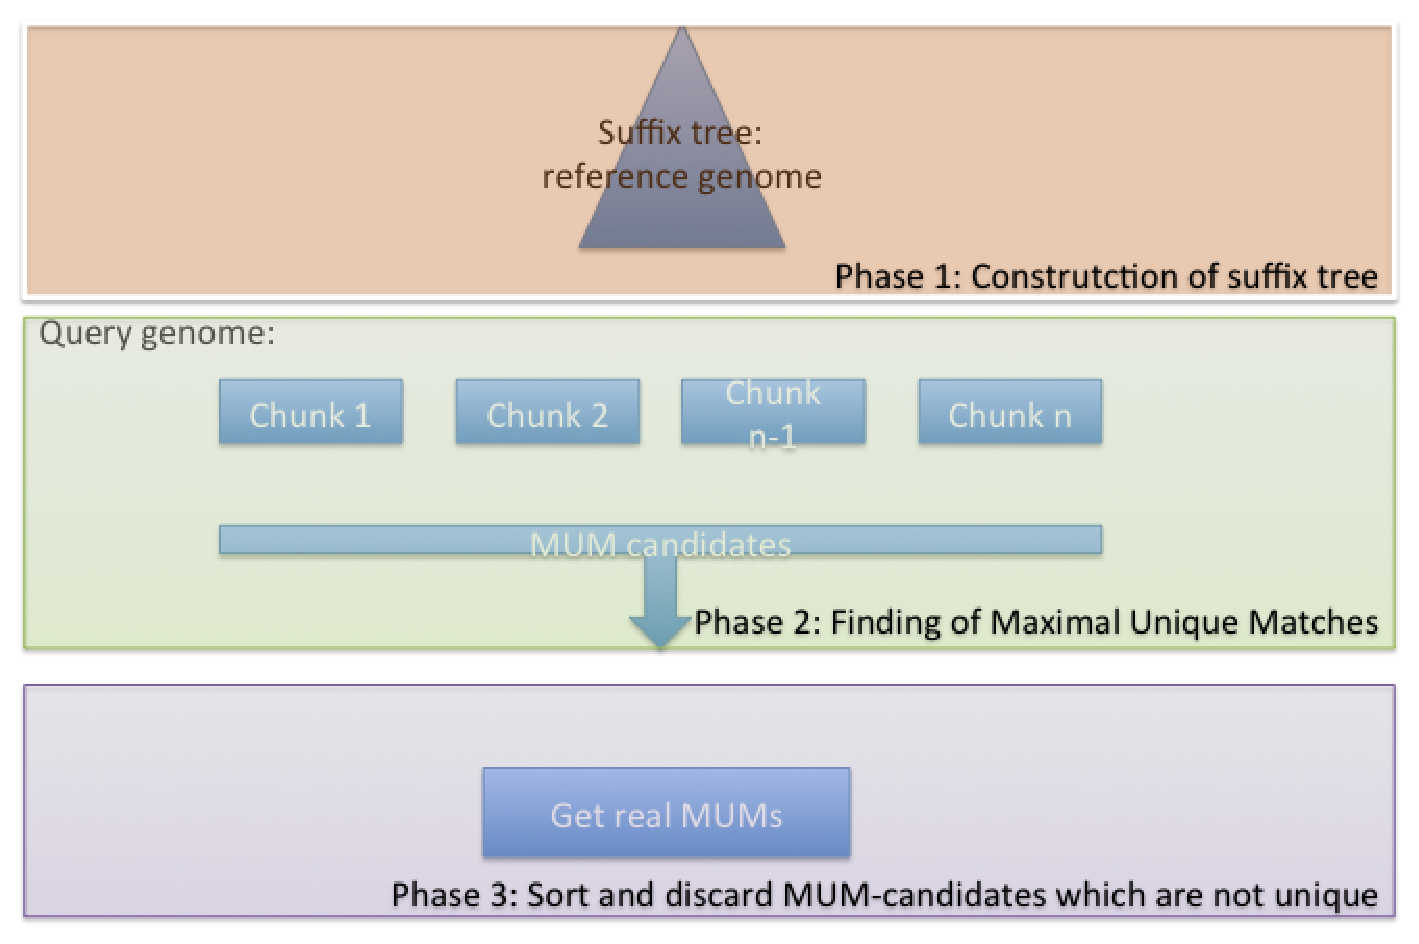
\epsfig{file=Phases.eps, height=1.5in, width=2in}
\caption{Our approach is divided in three phases: Splitting query genome data (chunks) according to the number of available cores using 1 thread per core; Parallel execution of the search for MUMs for every chunk then every thread has its own list of MUM-candidates; and Get MUMs from every MUM-candidate list of all threads.}
  \label{phases}
\end{figure}
The division of Query genome  was used using the paradigm of data-level parallelism which consists of a generation of chunks of a query sequence with a fixed size. The chunk size was computed with Query genome length divided by number of available threads. To get a MUM, it requires an important feature its uniqueness. Uniqueness can only be found when a whole genome is checked, see Figure \ref{Whole-MUM}. If some part of it is only evaluated we could miss the rest of the genome. In other words, after finding MUMs within a chunk it is not possible to determine if the MUM found is or not a "unique" MUM, globally in the query genome,  because these MUMs are unique only in the chunk that has been read, the rest of the genome it is not known until all query genome has been read. In Figure \ref{Whole-MUM} is shown the consequences of using chunks for query genome. Meanwhile we may speed up the MUM search we need to deal with the discard of MUM-candidates which are not a real MUM. So that, after finding all MUM-candidates for every thread we need to verify which of MUM-candidates are MUM.
\begin{figure}  
\centering 
  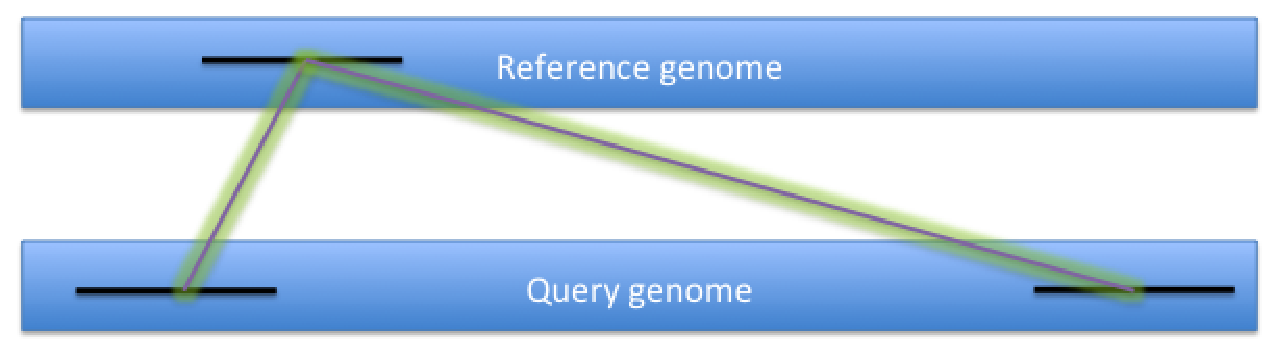
\epsfig{file=Whole-MUM.eps, height=1in, width=2in}
\caption{MUM in reference genome but not in query genome.} 
\label{Whole-MUM} 
\end{figure}
In Figure \ref{phases} we can see phase 3 which involves to extract the list of MUM from the set of MUM-candidates of every chunk in the query genome. In order to get the real MUMs we filter MUM-candidates that are overlapped by bigger MUM-candidates.
\section{Results}
%\begin{table}
%\centering
%\caption{Frequency of Special Characters}
%\begin{tabular}{|c|c|l|} \hline
%Non-English or Math&Frequency&Comments\\ \hline
%\O & 1 in 1,000& For Swedish names\\ \hline
%$\pi$ & 1 in 5& Common in math\\ \hline
%\$ & 4 in 5 & Used in business\\ \hline
%$\Psi^2_1$ & 1 in 40,000& Unexplained usage\\
%\hline\end{tabular}
%\end{table}

%\begin{table*}
%\centering
%\caption{Some Typical Commands}
%\begin{tabular}{|c|c|l|} \hline
%Command&A Number&Comments\\ \hline
%\texttt{{\char'134}alignauthor} & 100& Author alignment\\ \hline
%\texttt{{\char'134}numberofauthors}& 200& Author enumeration\\ \hline
%\texttt{{\char'134}table}& 300 & For tables\\ \hline
%\texttt{{\char'134}table*}& 400& For wider tables\\ \hline\end{tabular}
%\end{table*}
% end the environment with {table*}, NOTE not {table}!

%\begin{figure}
%\centering
%\epsfig{file=fly.eps, height=1in, width=1in}
%\caption{A sample black and whte graphic (.eps format)
%that has been resized with the \texttt{epsfig} command.}
%\end{figure}


%\newtheorem{theorem}{Theorem}
%\begin{theorem}
%Let $f$ be continuous on $[a,b]$.  If $G$ is
%an antiderivative for $f$ on $[a,b]$, then
%\begin{displaymath}\int^b_af(t)dt = G(b) - G(a).\end{displaymath}
%\end{theorem}

%\begin{figure*}
%\centering
%\epsfig{file=flies.eps}
%\caption{A sample black and white graphic (.eps format)
%that needs to span two columns of text.}
%\end{figure*}
 
%\begin{proof}
%Suppose on the contrary there exists a real number $L$ such that
%\begin{displaymath}
%\lim_{x\rightarrow\infty} \frac{f(x)}{g(x)} = L.
%\end{displaymath}
%Then
%\begin{displaymath}
%l=\lim_{x\rightarrow c} f(x)
%= \lim_{x\rightarrow c}
%\left[ g{x} \cdot \frac{f(x)}{g(x)} \right ]
%= \lim_{x\rightarrow c} g(x) \cdot \lim_{x\rightarrow c}
%\frac{f(x)}{g(x)} = 0\cdot L = 0,
%\end{displaymath}
%which contradicts our assumption that $l\neq 0$.
%\end{proof}

\section{Conclusions}
%\end{document}  % This is where a 'short' article might terminate

%ACKNOWLEDGMENTS are optional
\section{Acknowledgments}
This work was supported by grant from Ejecuci\'on eficiente de aplicaciones multidisciplinares: nuevos desaf\'ios en la era multi/many core, with reference TIN2011-28689-C02-01.
%
% The following two commands are all you need in the
% initial runs of your .tex file to
% produce the bibliography for the citations in your paper.
\bibliographystyle{abbrv}
\bibliography{mum-mc}  % sigproc.bib is the name of the Bibliography in this case
% You must have a proper ".bib" file
%  and remember to run:
% latex bibtex latex latex
% to resolve all references
%
% ACM needs 'a single self-contained file'!
%
%APPENDICES are optional
%\balancecolumns
\balancecolumns
% That's all folks!
\end{document}
